\section{Introduction}\label{sec:introduction}


\subsection{Overview}\label{sec:overview}
This chapter provides describes methods which are used in this research.
The main goal of the thesis is to figure out how Apache Flink and Kafka Streams
behave, perform, what kind of configurations are needed, how do solve fault tolerance problems
in case of a stateful streaming.
They both are designed for using in a streaming domain but there must be some difference
about how do they perform and get configured to run them in Kubernetes cluster.
The key moments for both systems are: scalability, resilience, fault tolerance, cost efficiency,
setup complexity, documentation, learning curve.

In order to get experiments running it is crucial to get an execution environment, especially
for a big data solutions which is not possible to run on a laptop.
Big data solutions and benchmarks require a cluster of hardware machines which represents node.
For this reason all the benchmarks and execution environment is done with AWS and EKS in
particular.
AWS provides such service as Amazon Managed Streaming.
Obviously it solves a lot of configuration problems, but adds additional cost.
It should be suitable for less loaded streaming solutions where load demand is not that big
and there's no dedicated team.
Really heavy loaded services where latency is also is important rely on their own
Kafka cluster setup and streaming setup such as Spark Streaming or Apache Flink.
These experiments are based on custom configuration provided by Theodolite framework.
Theodolite provides essential customizable Kafka cluster setup which is easily to reconfigure
and have more control over running experiments which makes also easy deployable cluster
for EKS infrastructure.

In order to get a measurable benchmarks, Theodolite provides a superb framework to get
things running and measurable with the following tools: Grafana, Prometheus Operator.
These tools have out of the box ready and configurable prometheus pod monitoring agents
to get any kind of metrics from running pods within the EC2 node.
Also, Theodolite operator as well as Prometheus and Grafana are easily deployable
are designed specifically for Kubernetes cluster environment which provides a super low latency
real time metrics.

One of the most important step is a data analysis, which is also possible using Theodolite framework
since it provides metrics export interface.
All the recorded metrics will be analysed using Python libraries and tools.


\subsection{Research Objectives}\label{sec:research-objectives}
Since Apache Flink and Kafka streams are supposed to solve data streaming problems, it's
quite important to understand their scalability efficiency for a highly loaded systems.
While this research was being done, another important event happened is a release of Java 21
and support for the brand new Generational ZGC which is an experimental low-latency JVM
Garbage Collector.
It's fascinating if the new JVM Garbage Collector is able to add any performance boost for
stateful streaming use case, and is there any performance advantages comparing to Java 11
and Java 21 without ZGC.
As a conclusion there following sub problems:

\begin{description}
    \item[Performance comparison] Experiments with Flink and Kafka Streaming running on Java 11,
    Java 21 and Java 21 with ZGC.
    \item[Scability experiments] How do Flink and Kafka Streams perform with different Java versions
    in case of a resource shortage, for example a shortage of replicas in case of a high load.
    \item[Fault Tolerance] What if highly loaded streaming pipelines get replicas killed, how
    would react Flink and Kafka Streams, how much time they need to restore a state and how consumer
    group latency would look like.
    kafka consumer group latency is especially crucial since it defines how fast the system
    is able to react on specific events, like a fraud detection.
\end{description}

Besides the sub problems above, there are additional questions about cloud configuration for Flink
and Kafka Streams, since Flink requires additional steps to get the Flink cluster running.
Especially it's fascinating with the brand new Flink Kubernetes operator release.
It supposed to dramatically simplify operations of the Flink cluster, and it's cloud configuration.
Moreover, the latest Flink Kubernetes Operator release supports the autoscaling functionality out of the box.

%\newpage
%
%
%
%\newpage


\section{Experimental Setup}\label{sec:exp-setup}
This section covers an infrastructure setup for experiments.
It must be said that setting up a working infrastructure was the most
challenging part of the thesis, however despite on a fact that a goal
of the thesis is a comparison of two powerful data streaming frameworks,
their cloud setup is incredibly challenging.
Developer or a researcher is supposed to know quite well Kubernetes infrastructure,
its principles, challenges, common problems and incoming errors.


\subsection{EKS Cluster Configuration}\label{subsec:eks-cluster-configuration}
EKS provides a decent infrastructure in order to get started with the
Kubernetes cluster.
Obviously that is not free, but it's well documented and quite easy
to get started with a template configuration.
The first EKS cluster for experiments was created manually, but following
standard steps.
It works for the first time, but recreation of EKS cluster gets extremely
tedious once it's needs to be ofter created and deleted.
EKS cluster should not be running while there is no any experiments running, since
it gets extremely costly, especially if EKS is used for scalability testing.
Fortunately, such problem is quite common for devops engineers and for this
reason there are superb tools already available for such use cases.
The most popular are Terraform and eksctl.
Despite on the fact that eksctl is specifically designed for EKS cluster, Terraform
provides more configurable API not only for EKS but for Kubernetes as well which
makes it and excellent for deploying and destroying cluster infrastructure
with a few commands.

\begin{lstlisting}[label={lst:eks-example}]
resource "aws_eks_cluster" "my-eks-cluster-name" {
  kubernetes_network_config {
    ip_family         = "ipv4"
    service_ipv4_cidr = "10.100.0.0/16"
  }

  name     = "my-eks-cluster-name"
  role_arn = "arn:aws:iam::112233:role/MyClusterRole"

  tags_all = {
    "team" = "taltech"
  }

  version = "1.28"

  vpc_config {
    endpoint_public_access  = "false"
    public_access_cidrs     = ["0.0.0.0/0"]
    security_group_ids      = ["sg-group-id"]
    subnet_ids              = ["subnet-id-1", "subnet-id-2"]
  }
\end{lstlisting}

The code snippet above ~\ref{lst:eks-example} shows Terraform script to
create EKS cluster with running a single command.



\subsection{Deployment with Terraform}\label{subsec:deployment-with-terraform}
As it was mentioned earlier, Terraform allows a developer to automate
operations with EKS cluster using a code.
There is a specific term for it, which is IaC.
Having a complex Kubernetes cluster setup it's extremely tedious and error-prone
getting services running in the EKS, especially with an increasing code base.
Terraform provides a readable for human and computer configuration, where a developer
defines which cloud resources must be created after running Terraform scripts.
It's also needs some time to learn a docs and then get scripts running.
The way Terraform scripts were initiated is using another popular tool which is
the terraformer.
This tools is an open source program provided by Google which is able to scan a currently
running infrastructure of a cloud provider like AWS and created based on it a
structured Terraform scripts which will be an entry point to maintain the EKS.
Specially for these benchmarks it is important to specify node groups
for different services which must be able to scale independently, by increasing
a number and a type of EC2 node.
For example the load generator service must not run on the same node as the Kafka cluster,
to make sure there's no impact on Kafka cluster or any other service.

In general, via Terraform is possible to define cloud resources, and get them deployed with
scripts.
Any specific details are available in docs.
The core infrastructure which is needed for running benchmarks is a different node groups with node types,
because some service consumer different types of node parameters.

\begin{lstlisting}[label={lst:ter-kafka}]
resource "aws_eks_node_group" "kafkaNodeGroup" {
  ami_type       = "AL2_x86_64"
  capacity_type  = "ON_DEMAND"
  cluster_name   = aws_eks_cluster.my-eks-cluster.name
  instance_types = ["d2.xlarge"]

  taint {
    key = "type"
    value  = "kafka-node"
    effect = "NO_SCHEDULE"
  }

  labels = {
    type = "kafka-node"
  }

  node_group_name = "kafkaNodeGroup"
  node_role_arn   = "arn:aws:iam::112233:role/MsThesisNodeRole"

  scaling_config {
    desired_size = "3"
    max_size     = "3"
    min_size     = "3"
  }

  subnet_ids = ["subnet-id-1", "subnet-id-2"]

  version = "1.28"
}
\end{lstlisting}


The code snippet above ~\ref{lst:ter-kafka} shows a base Terraform script on order to create
a node group for EKS cluster.
Such script creates a node group of 3 nodes of type d2.xlarge which is sufficient to deploy and run
Kafka cluster with 3 brokers.
However, it's possible to run multiple brokers on a single EC2 node, but for experiments
each broker run only on a separate node to make predictable and balanced cpu, memory, and disc
resources consumption.
The node type d2.xlarge is suggested to be used for nodes without Amazon EBS by Confluent.
Since experiments are not supposed to be running 24/7 in production, it's sufficient to take node
with internal storage.


\begin{table}[h]
    \centering
    \begin{tabular}{@{}ll@{}}
        \toprule
        Specification          & Detail                       \\ \midrule
        Instance Type          & d2.xlarge                    \\
        vCPUs                  & 4                            \\
        Memory                 & 30.5 GiB                     \\
        Network Performance    & Moderate                     \\
        Physical Processor     & Intel Xeon E5-2676 v3 (Haswell) \\
        Clock Speed            & 2.4 GHz                      \\
        CPU Architecture       & x86\_64                      \\
        EBS Optimized          & True                         \\
        Max Bandwidth          & 750 Mbps on EBS              \\
        Max I/O Operations/sec & 6000 on EBS                  \\
        Disk Space             & 2048 GiB                     \\
        Elastic Map Reduce     & Supported                    \\
        Pricing                & Starting at \$0.69 per hour  \\ \bottomrule
    \end{tabular}
    \caption{AWS EC2 d2.xlarge Instance Specification}
    \label{tab:d2_xlarge_spec}
\end{table}

The Table~\ref{tab:d2_xlarge_spec} above shows detailed specification, 2TB of disc space is more than
enough to run benchmarks for a short period of time.
The price for such cluster is about \$2 per hour.
If the benchmarks takes 4 hours, then price for such Kafka cluster is \$8.


\newpage

\begin{figure}[H]
    \centering
    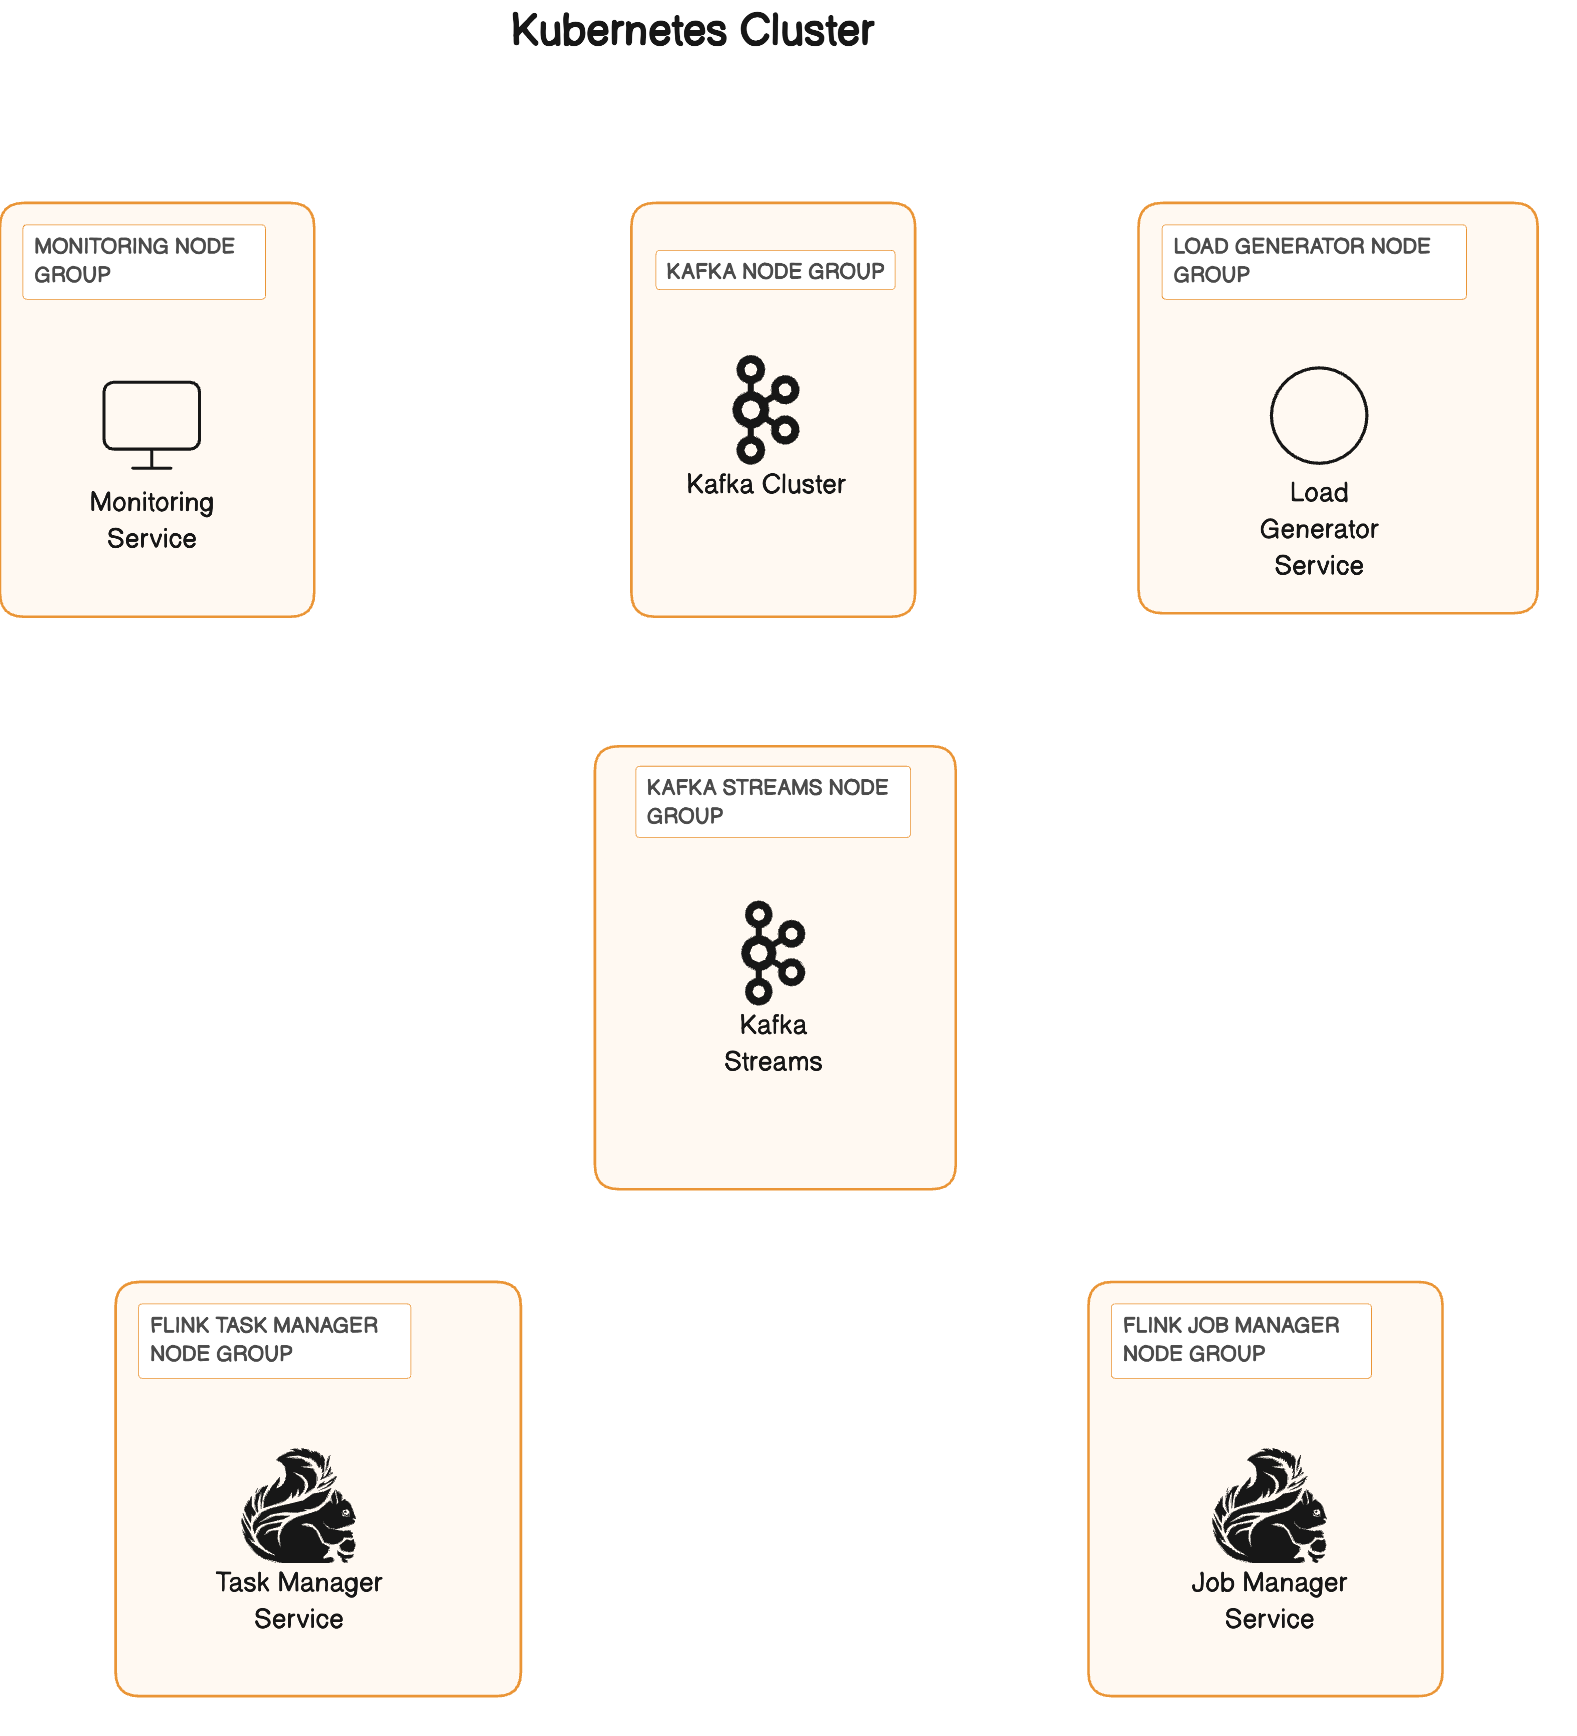
\includegraphics[width=0.9\textwidth]{figures/eks-node-groups}
    \caption{\textit{Node groups which were used for experiments.}}
    \label{fig:eks-groups-img}
\end{figure}


\subsection{Node Groups Configuration}\label{subsec:node-group}
In a previous chapter was given a brief overview over Kafka cluster node group,
but this chapter will give an overview over rest of the EKS cluster components.


\subsubsection{Load Generator}
The load generator is only designed to generate a stream of Kafka messages, where
each message is a random byte array of 1KB size.
The generator is based on a simple spring boot app, where the load of messages is
generated with ScheduledThreadPoolExecutor of 4 threads.
A nature of the mode generator requires more cpus rather than a disc space.

The node group of the generator consists only of a single node of a type m6i.xlarge.
This node is efficient enough to generate 200K MPS and even much more.

\subsubsection{Kafka Streams}
Kafka Streams as well as the load generator is based on Spring Boot framework since it is
the mose popular and common framework for running Java applications and provides out of the box
support for Kafka Streams.
It's important to have as fewer configurations as possible to simply run and Deploy Kafka Steams
instance.
Kafka Steams node groups consists of m6in.xlarge type nodes.

\subsubsection{Apache Flink}
Apache Flink requires a different approach for node groups comparing to Kafka Streams since
it has a different architecture and includes additional components to run and manage streaming
jobs.
For this benchmarking experiments two separate node groups were used.
The first one of for Flink job manager and the second one is for Flink task managers which
are workers.
Flink job managers require much less resources since they are intended to control task managers.
For these experiments for task managers was chosen a node groups of type t3.medium.
For task managers was chosen a more performant node type m6in.xlarge.
The same type was used for Kafka Streams to compare a resource consumption for two solutions.

However, these experiments required additional component for the Flink cluster which is
Flink Kubernetes Operator.
It is open source and open source solution to dramatically simplify a Flink cluster management.
For experiments, it was running withing the monitoring node group since it doesn't consume
many resources.

\subsubsection{Monitoring}
The following group was used as a default node group for any other services, like Prometheus,
Grafana, Prometheus Operator, Flink Operator.
Monitor node groups consists of two nodes of type t3.medium.

\subsection{Infrastructure as Code}\label{subsec:infrastructure-as-code}
With such complex cloud setup, it's simple not possible to create and such
complex infrastructure and fortunately there are available tools for such use cases.
The main tools which were used for experiments are \textbf{Helm} and \textbf{kubectl}

\begin{description}
    \item[Helm] is a tool which manages packages for Kubernetes cluster, it allows to create,
    update and deleted Kubernetes resources.
    \item[kubectl] is a cli tools which also allows to manage resources, but not as a package but
    rather each resource separately.
\end{description}

For experiments, were create all required Kubernetes resources which makes deployment
quite fast and efficient.

For each experiment there's a set of Kubernetes resource files which is used
for a specific benchmark.
It makes deployment easier and less error-prone, however it might bring
too much boilerplate code.



\section{Implementation Details}\label{sec:implementation-details}
This section covers use case implementation with Kafka Streams and Apache Flink.
The source code for Apache Flink and Kafka Streams is Java Gradle based project,
where gradle version is 8.5 and jar were build with Java 11 and Java 21.
Both builds were deployed to Amazon ECR, such that once deployed Docker images
are reusable and not required to be built for each experiment separately.
The core image built platform is Docker.
In order to deploy build images two cli tools were used.

\begin{description}
    \item[Docker cli] is a tool which help to build Docker images with the app and deploy them
    to Kubernetes cluster.
    Quite important to use a correct platform, for experiment were chosen Linux distros, for
    this reason the following build parameter was used --platform=linux/amd64.
    Moreover, docker cli provide aws login system which knows how to deploy build images directly to
    Amazon ECR.
    \item[aws cli] is a cli which provides API to work with AWS resources, docker cli
    is integrated with the aws cli quite well.
\end{description}


%\begin{lstlisting}[label={lst:ecr-example}]
%aws ecr get-login-password --region aws-region-name |
%docker login --username AWS --password-stdin aws-account-id
%docker buildx build -t ecr-name . --platform=linux/amd64 --push
%\end{lstlisting}

%The code snippet above ~\ref{lst:ecr-example} is an example of how to deploy built docker image
%to ECR for linux/amd64 platform.

%\newpage

\subsection{Rule Based Matcher}\label{subsec:rule-matcher}

\begin{figure}[H]
    \centering
    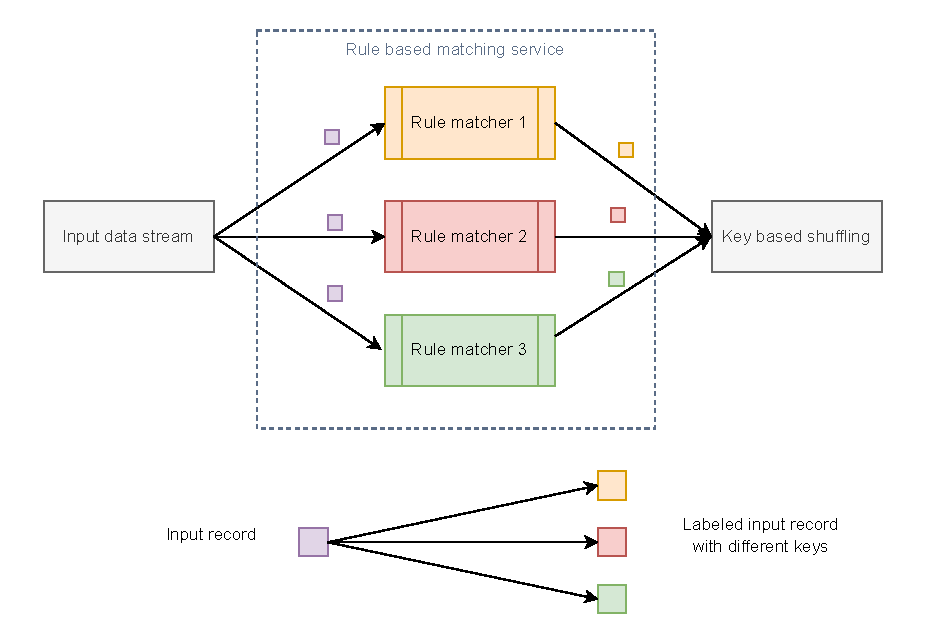
\includegraphics[width=1\textwidth]{figures/rule-matcher}
    \caption{\textit{Rule based matcher.}}
    \label{fig:rule-matcher}
\end{figure}

This is the core component of streaming pipeline for the use case.
It could be considered as a black box which provides a single api method to match
incoming bytearray record.
Its logic could be described using diagram above ~\ref{fig:rule-matcher}.

The matched has a single method interface for byte array record which
can based on defined rules is able to matched with them.
All matched rules get shuffled by name which makes to distributed
further processing among all replicas.
The main parameters of the matcher are selectivity and number of rules.

\begin{description}
    \item[Matching Rule] is a rule which has a selectivity property to be matched with a byte array record.
    \item[Selectivity] is a value with a floating point which defined a probability witch record can be
    matched.
\end{description}

For example, if the matcher has 10000 rules, with selectivity of 0.00002, then a probability with
which it will be matched with incoming record is 0.00002\%.
These values could be different depending on a system simulation.
The matcher is a prototype which is supposed to simulate a real service.
Since the rule matched is not a focus of the research, it is more than enough to use
a prototype.

\subsection{Kafka Streams Implementation}\label{subsec:kafka-streams-implementation}

\begin{figure}[H]
    \centering
    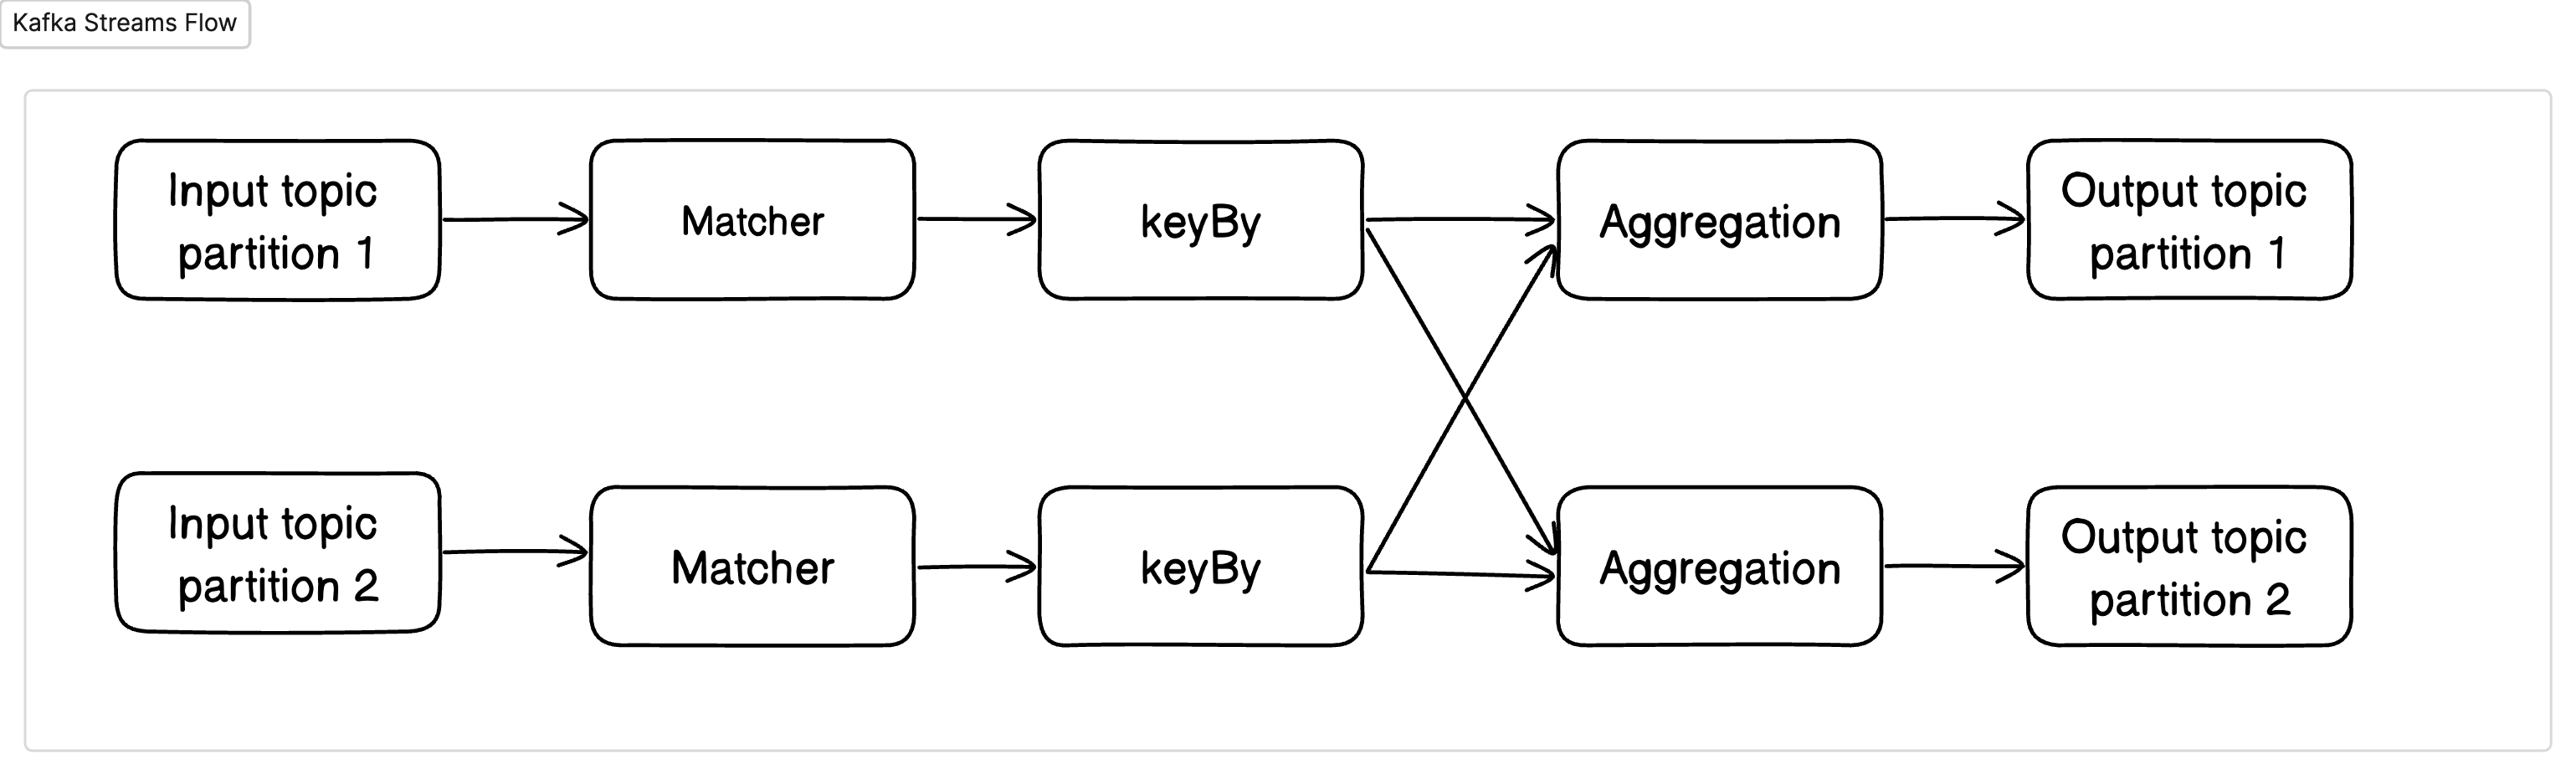
\includegraphics[width=1\textwidth]{figures/k-streams-shuffle}
    \caption{\textit{Kafka Streams flow.}}
    \label{fig:k-stream-shufle}
\end{figure}

Kafka Streams flow is presented on the figure above ~\ref{fig:k-stream-shufle}.
For the experiments Kafka Streams use default configurations with Kafka
commit time period of 30 seconds.


\subsection{Flink Implementation}\label{subsec:flink-implementation}

\begin{figure}[H]
    \centering
    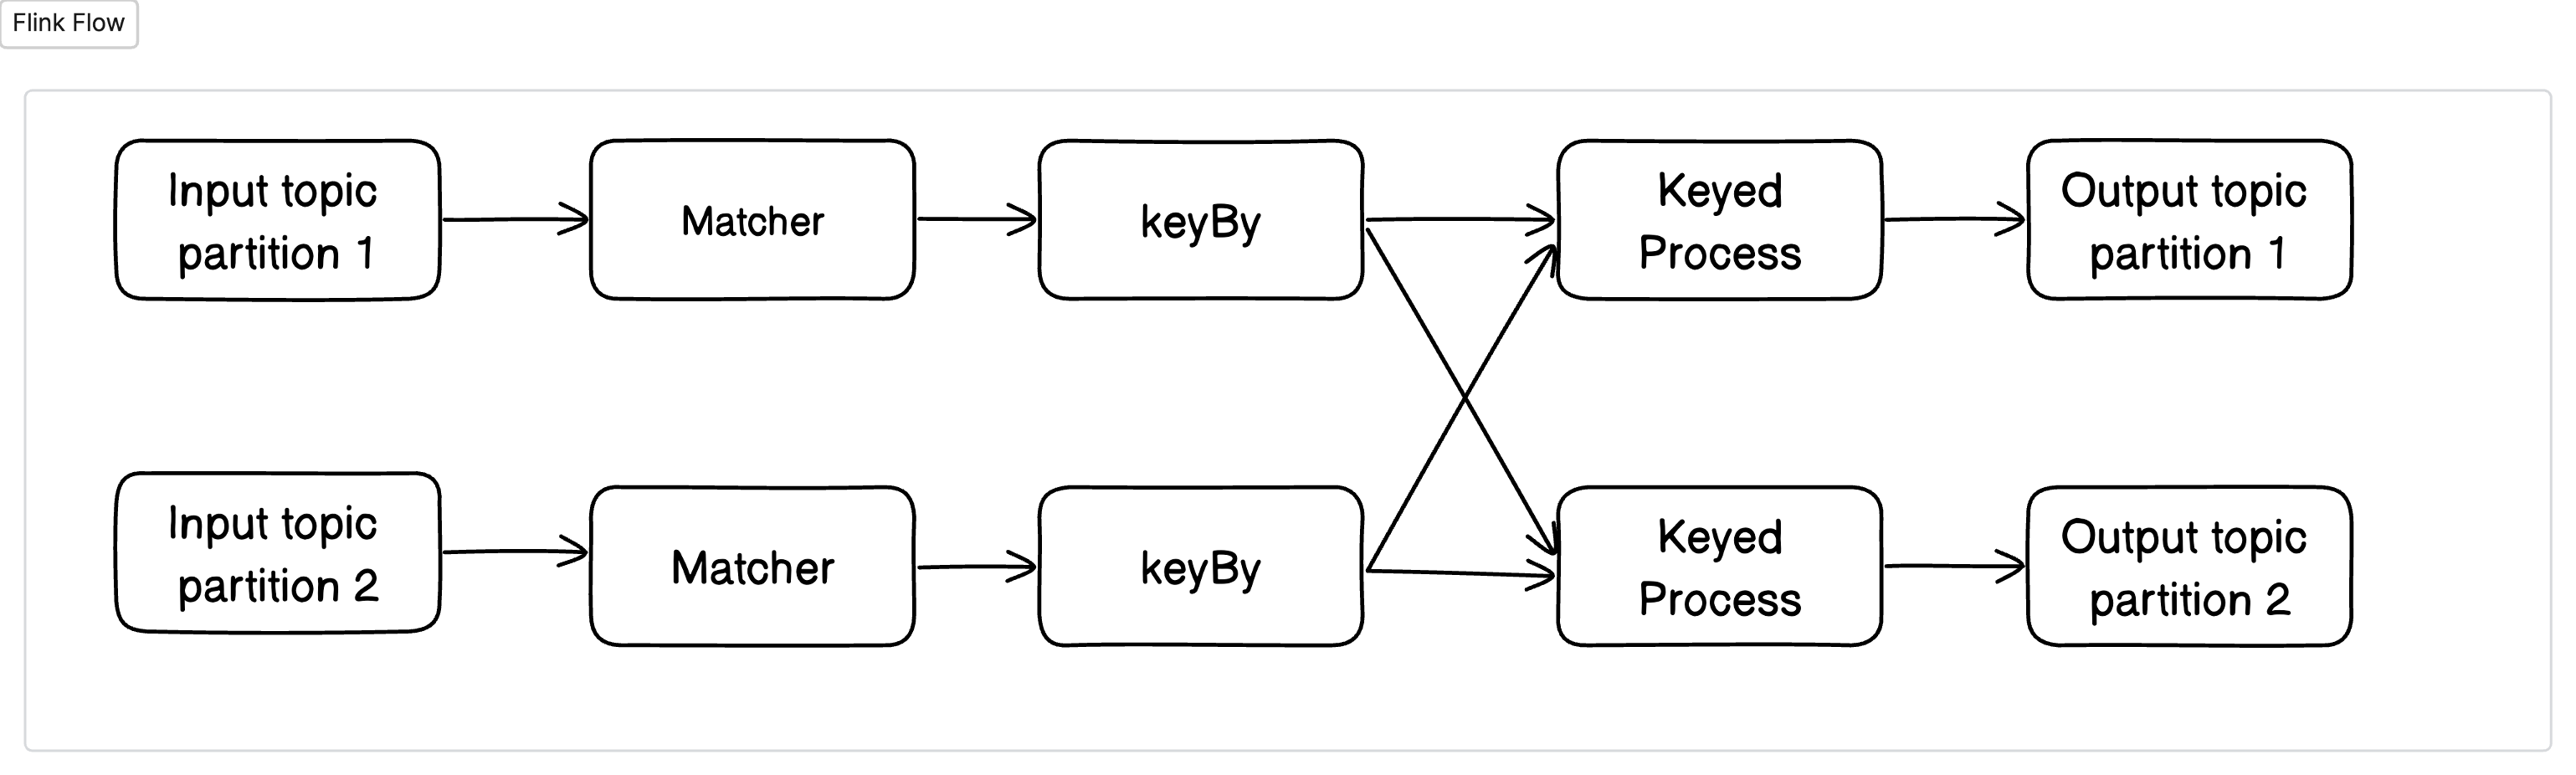
\includegraphics[width=1\textwidth]{figures/flink-shuffle}
    \caption{\textit{Flink flow.}}
    \label{fig:flink-shuffle}
\end{figure}

Flink is using keyed process which also type of aggregation but with a little
bi different behaviour.
Flink implementation uses checkpoints, which are get saved every 30 seconds
to Amazon S3 storage.
It was done to get the Kafka commit interval like in
Kafka Streams implementation.
The same commit interval helps to compare a performance difference.

However, experiments with Flink require to install to EKS cluster additional
dependencies which are need to manager Flink cluster.
These tools are: cert-manager for Kubernetes cluster, Flink Kubernetes Operator,
RBAC roles and permission for Flink Operator which must be allowed to
deploy Flink task managers and job managers.


\section{Monitoring}\label{sec:monitoring-and-benchmarking-setup}
Monitoring consists of two main component which are Grafana and Prometheus.
Prometheus is a time series database which is optimized for fast
and frequent queries which give information about different kind of
available metrics.
Since Prometheus is a centralised data storage, there are configurable
Prometheus exporters which know how to read metrics from running pods
in the same node.
There are different kinds of metrics options available, one of them
is JMX exporter, which is common java bases services.
There's available open sourced Prometheus Kafka exporter which requires
minimal configurations to get Kafka cluster metrics exporter to Prometheus.

Grafana provides UI interface to configure a datasource which is Prometheus
for experiments flow.
For each individual metric, is PromQl under the hood which periodically
request Prometheus for continuous time services charts.
Query request frequency is a fast enough to make metrics a real time.
This base setup is enough for experiments, however in a future research
additional tools will be required.


\section{Theodolite Framework}
Theodolite is a framework for benchmarking the horizontal and vertical scalability
of cloud-native applications in Kubernetes.
Native Kubernetes support makes it an excellent tool for experiments
since EKS cluster is used.
Theodolite provides documented examples of how to create Kubernetes resources
in order to run benchmarks with less effort, everything is automated.
However, it might take some time to get confident with configuring
benchmarks for different use cases.
Besides a provided out-of-the-box tools like Kafka cluster, Grafana, Prometheus,
Theodolite also contains an operator which manages benchmarks deployment,
configurations and runtime.

For each experiment there is set of Kubernetes resource files which get installed
with one sh file.

\subsection{Experiment Lifecycle}\label{subsec:experiment-lifecycle}
Before running the experiments, it's important to make sure that all required
dependencies are installed before start.
Experiment lifecycle could be described in a several steps.

\begin{description}
    \item[Deployment of benchmark executer] is a first manual step which tells Theodolite
    with what parameters deploy the system.
    For example, number of replicas, load generator MPS, number of experiment executions,
    execution time, pause time between experiments.
    \item[Execution start] is an automatic action managed be the Theodolite operator which starts
    load generator instances and Flink/Kafka Streams instances.
    \item[Execution] is defined period of time when deployed instances are running in their
    native mode.
    \item[Execution stop] once time has elapsed, Theodolite operator saved recorded metrics to csv files.
    \item[Execution reset] if there are configured multiple experiments, then
    Theodolite operator waits for defined period of time to start a new experiment.
\end{description}

Everything is automated besides deployment of benchmark executer.

\subsection{Performance Metrics}\label{subsec:performance-metrics}

The results will be provided as visual illustration having additional metrics like:

\begin{description}
    \item[Kafka consumer group lag] Consumer group represents a set of Kafka consumers
    united into one big consumer group.
    Such metric defines how efficient the system is able to process an incoming load of
    kafka messages from the input topic where the indicator of processed messages is Kafka topic
    offset.
    If the system as a consumer group has committed only 5 messages of 10 then the lag is going to grow.
    And vice versa, if a consumer group has committed 15 messaged out of 10 incoming then it means that
    the system has been able to process previously arrived messages and the lag is going to go down up to
    zero, which means there is no lag anymore.
    It will be seen as a slope on a time series metric.
    \item[Input message rate]
    this metric shows how many messages the system as the consumer group has received during a certain period of time.
    It could be measured using Kafka Prometheus exporter and PromQL.
    \item[Output message rate]
    This metric shows how many messages the system has produced during a certain period of time, and
    also could be measured using PromQL.
\end{description}

For the following experiments, both Flink and Kafka Streams use 30 seconds
topic commit period.
It needs to be clarified that this research is not focusing on cpu and heap consumption,
due to additional technical difficulties and cloud configuration.
Such metrics will be definitely included in the next performance evaluation.
But still there were cpu limits applied for Flink task manager pods.
Each replica could use up to the 1 cpu, but there were no limits applied
for Kafka Streams replicas.
Kafka Steams replicas used EC2 node cpu limitations due
to errors during deployment with having limit of 1 cpu.
This needs to be researched as well as a next step.


\subsection{Data Collection}\label{subsec:data-collection}
Since for experiments Theodolite framework is used, it provides data collection api.
For each experiment, it is possible to define a set of PromQL queries which
will be executed once the experiment has finished benchmark execution.
During the experiment all the data gets collected to Prometheus as time
series metrics which will be read and saved to the Kubernetes volume as
csv files.
Once csv files are saved, it's possible to download them on a personal
computer for a further analysis.
